\chapter{Big Data challenges in astronomy} % \chapter{Astronomy Big Data}
\label{theproblem}

Astronomical datasets are growing at an exponential rate: the next generation of telescopes will collect data at rates of
several terabytes % terabytes
per day. This data
deluge % , now and int the future,
presents some critical challenges for the way astronomers
can
get new knowledge from their data.
These extremely large datasets, or datasets with high data rates, are commonly known as
\emph{Big Data}.

Big Data are high-volume, high-velocity, and/or high-variety information assets that require new forms of processing to enable enhanced
decision making\footnote{for instance, fast follow up of transients in the data collected by the LSST}, % decision making,
insight discovery and process optimization. Examples of big data
outside of astronomy
include information such as Web search results, electronic messages (e.g. SMS, email and instant messages), social media postings, pictures, videos, 
or large web % and 
system log data.
% However, it can also include cash transactions, check images, receipts and other transactional information depending on the source of the information.
These situations require the % This situation requires
processing of terabytes and even petabytes of data. This is achieved by
means of
 distributed processing.
% This is one of major reasons for the power of Web companies such as Google, Amazon or social networks like Facebook and Twitter.
% Relational databases
Relational Database Systems (RDBMS)
are found to be inadequate in distributed processing involving very large number of servers and handling Big Data applications, due to the limitations of query speed, storage size, and scalabilty inherent to the tasks of keeping relationships between database tables, atomicity of transactions, and the storage layout of data in disk.

% In this chapter, we make an overview of some of the greatest telescopes and the amount of data they acquire and store.

In the next sections, we will review some of the current and future challenges for astronomical data processing, which justify the search for NoSQL solutions for astronomical data sharing.

% \section{Atacama Large Millimiter Array}
\section{The Atacama Large Millimetre/Submillimetre Array}

The Atacama Large Millimetre/Submillimetre Array (ALMA) % ALMA
is a worldwide project, % ; the synthesis of early visions of astronomers in its three partner communities: Europe, North America and Japan. It is a fusion of ideas, with its roots in three astronomical projects: the Millimeter Array (MMA) of the United States, the Large Southern Array (LSA) of Europe, and the Large Millimeter Array (LMA) of Japan.
built cooperatively by the European Southern Observatory (ESO), the National Radio Astronomical Observatory (NRAO) of the United States of America, and the National Astronomical Observatory of Japan (NJAO), in collaboration with the Academia Sinica of Taiwan.

 \begin{figure}[tb]
 \centering
 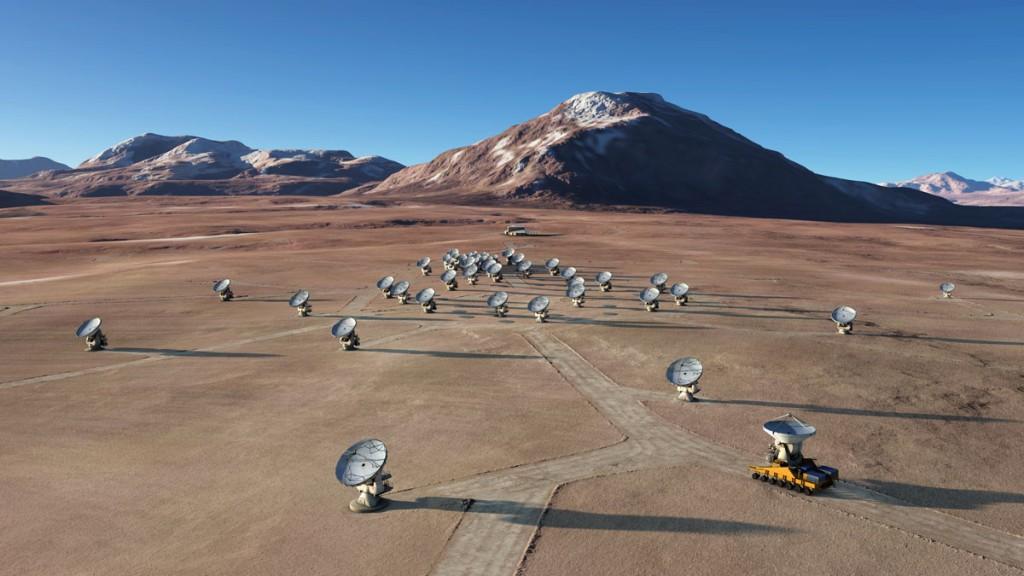
\includegraphics[width=\textwidth]{images/alma.jpg}
 % \caption{ALMA dishes in Atacama Desert}
 \caption{Artist's impression of ALMA dishes at the Chajnantor plateau, in the Atacama Desert}
 \end{figure}


ALMA
% is an instrument that
consists of a giant array of
sixty-six
12~m antennas with baselines up to
16~km,
and an additional compact array of
7~m
and
12~m antennas to greatly enhance ALMA's ability to image extended targets, located on the Chajnantor plateau at 5000m altitude.

%The design of
ALMA is driven by three key science goals:

\begin{itemize}

\item Detecting spectral line emission from CO in a normal galaxy like the Milky Way at a redshift of $z=3$, in less than 24 hours.

\item Imaging the gas kinematics in protostars and in protoplanetary disks around young Sun-like stars in the nearest molecular clouds ($150 pc$).

\item Providing precise high dynamic range images at an angular resolution of $0.1 arcsec$
\end{itemize}

In order to accomplish those goals,
% Initially, it will
ALMA will initially 
observe at wavelengths in the range $3 mm$ to
$400 \mu{}m$
($84$ to $720 GHz$). The antennas can be moved around, in order to
provide different % form arrays with different distributions of 
baseline lengths. More extended arrays
% will
give high spatial resolution,
while
more compact arrays give better sensitivity for extended sources. In addition to the array of
12~m
antennas, there is the Atacama Compact Array (ACA), used to image large scale structures that are not well sampled by the ALMA
12~m
array, consisting of twelve
7~m
antennas and four
12~m
antennas. 


The current ALMA Archive design allows for a maximum data rate of 64 MB/s and an average data rate
of 6.4 MB/s, which produces the long-term storage capacity of approximately 200 TB/year. The
ALMA correlators can
generate % producing a
data
up to 1000 MB/s. 

 
As stated in \cite{Etoka12}, the purpose of the ALMA archive is to provide services for:

\begin{itemize}

\item Persistent archiving and retrieval for observational data.

\item Search and retrieval of observations via several descriptors. % Observaction descriptors.

\item Retrieval of reduced datacubes
% Datacubes
produced by
the
pipeline.

\item Search and retrieval of technical and environmental data. % Technical and environmental data.
\end{itemize}

The main objective of the
ALMA Archive
conceptual design
is to guarantee that three ALMA Regional Centres (North America,
East Asia % Japan
and Europe) hold an identical copy of the archive at the Joint ALMA Observatory in Santiago. 

The
ALMA Front-end Archive
(AFA; the part of the archive directly accessed by the ALMA correlator)
is optimized for storage and preservation, not for data query and retrieval.

The ALMA Science Archive (ASA), on the other hand, is the user-facing part of the ALMA Archive. The ASA receives a transformed copy of the data from the AFA, because only a subset of the data and metadata in the AFA is considered to be queriable by the users.

% NOTA: desconectado del resto de la explicación
% ASA database is inspired from ObsCore, RADAMS and Hubble Legacy Archive plus Virtual Observatory Software:
% \begin{itemize}
% \item openCADC (\ref{opencadc}), which is used for database access and VO access protocol
% \item VOView, for Web components
% \end{itemize}

% TODO: Incluir 

\section{The Square Kilometre Array} % \section{Square Kilometer Array}

The Square
Kilometre % Kilometer
Array\urlnote{http://www.skatelescope.org/} (SKA) % Array (SKA)
is a global science and engineering project led by the SKA Organization, a not-for-profit company with its headquarters at Jodrell Bank Observatory, near Manchester. When construction starts in 2016 (according to
the official schedule\urlnote{http://www.skatelescope.org/the-project/project/}) % schedule)
in Australia and in Southern Africa, thousands of linked radio wave receptors will be located to combine the signals from the antennas in each region creating a telescope with a collecting area equivalent to a dish with an area of about one square kilometer to discover how the first stars and galaxies formed after the Big Bang, how galaxies have evolved and the nature of gravity. It comprises:

\begin{itemize}
\item An array of dish receptors in eight African countries. 
\item An array of mid frequency aperture arrays in the Karoo. 
\item A smaller array of dish receptors and an array of low frequency aperture arrays in the Murchison Radio-astronomy Observatory in Australia.
\end{itemize}

 \begin{figure}[tb]
 \centering
 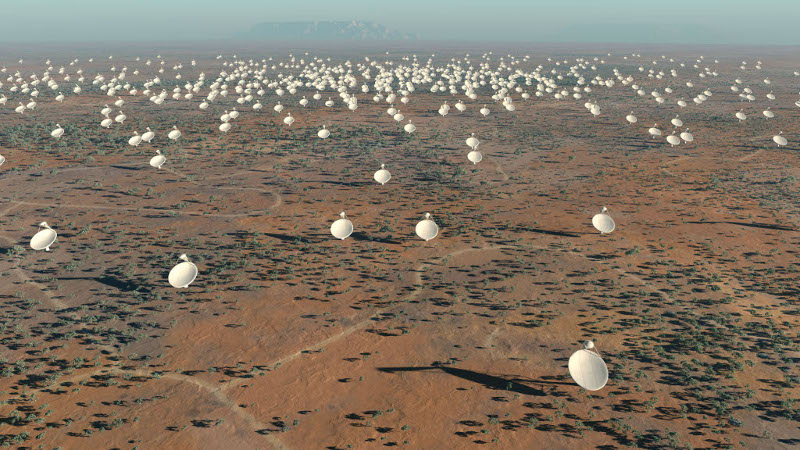
\includegraphics[width=\textwidth]{images/ska.jpg}
 \caption{Artist's impression of the SKA dishes. Credit: SKA Organisation/TDP/DRAO/Swinburne Astronomy Productions}
 \end{figure}

Some relevant figures and facts about SKA:

\begin{itemize}

\item The data collected by the SKA in a single day would take nearly two million years to playback on an ipod.
\item The SKA central computer will have the processing power of about one hundred million PCs.
\item The SKA will use enough optical fibre to wrap twice around the Earth.
\item The dishes of the SKA will produce 10 times the global internet traffic.
\item The SKA will generate enough raw data to fill 15 million 64 GB iPods every day.
\item SKA will be able to detect an airport radar on a planet 50 light years away.

\end{itemize}




\section{Murchinson Widefield Array}


The Murchison Widefield Array is the first Square Kilometre Array precursor to enter full operations, generating a huge amount of information that needs to be stored for later retrieval by scientists. To store the data generated by the MWA three 1 TB hard drives every two hours are needed (it will store about 3 Petabytes at the Pawsey Center each year), so the isn not just a matter of storing the observations but how to distribute them from the MWA team in remote places, like MIT, Victoria University of Wellington in New Zeahland and India. 

According to Professor Andreas Wicenec, from The University of Western Australia node of the International Centre for Radio Astronomy Research (ICRAR), SKA has ``now have more than 400 megabytes per second of MWA data streaming along the National Broadband Networ¡k from the desert 800 km away''. Data travels through a 10 gigabit per second connection between the Murchison Radio-astronomy Observatory (MRO) and Geraldton. \footnote{\url{http://www.skatelescope.org/news/pawsey-centre/}}

The data are not obviously intended to be fully available for everybody at every time: for instance, MIT researchers are interested in the early universe so filtering techniques to control what data is copied from the Pawsey Center archive to the MIT machines are used. By 2013, more than 150 TB of data had been transferred automatically to the MIT store, with a stream of up to 4 TB a day increasing that value. 




\section{Large Synoptic Survey Telescope}

The Large Synoptic Survey Telescope (LSST) is a new kind of telescope whose widefield of view allows it to observe large areas of the sky at once. It can take almost 1000 panoramic images each night, it can cover the sky twice a week. Data from LSST will be used to create a 3D map of the Universe with unprecedented depth and detail. Plans for sharing the data from LSST with the public are really ambitious, as it is intended that anyone with a PC can fly through the Universe, zooming past objects a hundred million times fainter than can be observed with the human eye. 

Some of the institutional members are Google, Caltech, Harvard-Smithsonian Center for Astrophysics, Fermi National Accelerator Laboratory or STSI. \footnote{For a full list of institutional members, browse to \url{http://lsst.org/lsst/about/members}}  


LSST observing will produce about 30 TB per night, leading to a total database over the ten years of operations of 60 PB for the raw data, and 30 PB for the catalog database, that will be processed using 100 TFlops. The data will be sent over existing optical fiber links from Chile to the U.S. 

Currently finishing the design and development stages, it is expected to start operating in 2022.